\section{Unsupervised Activity Representation}
Here we explain the generative model which we use in order to jointly learn the activities from videos. We start with explaining the basic notation we use in the model. We denote the $t^{th}$ frame of the $i^{th}$ video as $I^i_t$ and its subtitle as $L^i_t$. Moreover, we note the extracted frame representation as $y^i_t$. We model our algorithm based on activities and the note the activity of the $t^{th}$ frame of the $i^{th}$ video as $z^i_t$. Since our model is non-parametric, number of activities are not fixed and $z^i_t \in \mathcal{N}$.

\subsection{Beta Process Hidden Markov Model}
For joint clustering of time-series information, Fox et al.\cite{foxBPHMM} proposed the Beta Process Hidden Markov Models (BP-HMM) using the Indian Buffet Process\cite{ibp} of time-series sequences over features. It assumes that there exist a set of features which can explain the time-series corpus. Any of the time-series information exhibits a subset of available features. Here, we focus on videos as time-series information and feautures as activities similar to Hughes et al.\cite{npActivity}. We differ in the choices of the underlying distributions since we based our model on semantic multi-modal information, bag-of-visual-words and its Drichlet distribution is not applicable in our case.

In our model, each video $i$ chooses a set of activities through a activity vector $\mathbf{f^i}$ such that $f^i_k$ is $1$ if $i^th$ video has activity $k$, 0 otherwise. When the feature vectors of all videos in the courpus is concatanated, it becomes an activity matrix $\mathbf{F}$ such that $i^th$ row of the $\mathbf{F}$ is the activity vector $\mathbf{f^i}$. Moreover, each feature $k$ also has a activity frequency $b_k$  and a distribution parameter $\Theta_k$. Distribution parameter $\Theta_k$ is the base distribution of the feature distributions of the frames and it is beta random random variable since the frames has set of independent binary random variables. Moreover, in this setting, the activity paremeters $\Theta_k$ and $b_k$ follow the \emph{beta process} as;
\begin{equation}
  B|B_0,\gamma,\beta \sim \text{BP}(\beta,\gamma B_o), B=\sum_{k=1}^\infty b_k \delta_{\Theta_k}
\end{equation}
where $B_0$ and the $b_k$ are determined by the underlying poisson process \cite{hbp} and the feature vector is determined as independent Bernoulli draws as $f_{k}^i \sim Ber(b_k)$. After marginilizing over the $b_k$ and $\Theta_k$, this distribution is shown to be equivalent to Indian Buffet Process \cite{bpibp}. Where videos are customers and activities are dishes in the buffet. The first video chooses a $\text{Poisson}(\gamma)$ unique dishes. The following video $i$ chooses previously sampled activity $k$ with probability $\frac{m_k}{i}$ proportional to number of videos ($m_k$) chosen the activity $k$, and it also chooses $\text{Poisson}(\frac{\gamma}{i})$ new activities. Here, $\gamma$ controls the number of active features in each video and $\beta$ controls the likelihood of the features getting shared by multiple videos.

\begin{figure}[h!]
  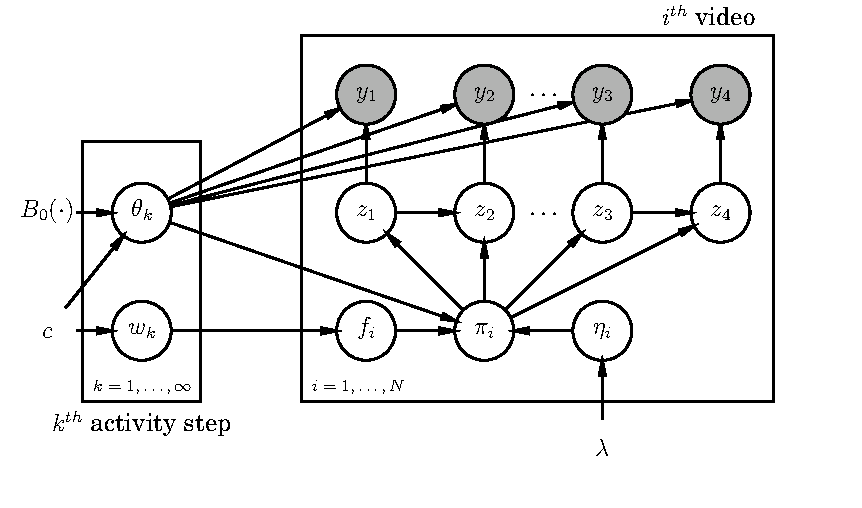
\includegraphics[width=0.5\textwidth]{plate}
  \caption{Graphical model for BP-HMM-O}
  \label{bphmmo}
\end{figure}


\subsection{Gibbs sampling for BP-HMM}
We employ Markov Chain Monte Carlo (MCMC) method for learning and inference of the BP-HMM. We base our algorithms on the MCMC procedure proposed by Fox et al.\cite{foxBPHMM}. It marginilizes over blah and blah and sample blah and blah. For faster convergence, we also utilize a series of data driven samplers. Here we only discuss the proposed data driven samplers and move the details of the remainin samplers to the Supplementary Material.

\paragraph{Data-Driven Sampler1}
\paragraph{Data-Driven Sampler2}
